\documentclass[12pt, letterpaper]{article}
\usepackage{times}
\usepackage{graphicx}
\usepackage{import}
\usepackage{fancyhdr}
\usepackage{wrapfig}
\usepackage[utf8]{inputenc}
\usepackage[hidelinks]{hyperref}
\usepackage{subcaption}
\usepackage{pdfpages}
\pagestyle{fancyplain}% <- use fancyplain instead fancy
\fancyhf{}
\addtolength{\headheight}{15pt}
\fancyhead[L]{Cyber Security - Konstantinos Poumpouridis}% <- added
\fancyhead[R]{488394}
\fancyfoot[C]{\thepage}
%\renewcommand\headrulewidth{0pt}% default ist .4pt
\renewcommand{\plainheadrulewidth}{.4pt}% default is 0pt
\title{Portfolio}
\author{Konstantinos Poumpouridis}
\date{03/03/2023}
\pagenumbering{arabic}
\begin{document}
\maketitle
\thispagestyle{empty}
\newpage
\section{Changelog}
    \begin{table}[htbp]
        \begin{tabular}{|l|l|l|}
            \hline
            Version & Changes         & Date   \tabularnewline \hline
            0.1     & Initial version & 07/05/23 \tabularnewline \hline
            0.2     & Added somebody & 30/05/23 \tabularnewline \hline
            0.3     & Added somebody & 13/06/23 \tabularnewline \hline
            0.4     & finished Portfolio & 14/06/23 \tabularnewline \hline
            0.5     & Added "What did you do?",  & 15/06/23 \tabularnewline \hline
            0.5.1     & Reworked sentence from we to I or me, expanded the conclusion of my progress & 15/06/23 \tabularnewline \hline
        \end{tabular}
    \end{table}
\newpage
\tableofcontents
\newpage


\section{Introduction}
\begin{itemize}
\item \textbf{What was your relevant prior knowledge and experience on security, Linux and networking or what did you do to obtain this knowledge?}
\hfill\break
\hfill\break
I'm from infrastructure and I used Ubuntu since 10.10 until I switched to macOS. So I had a basic understanding of Linux from the beginning. But the rest of the advanced knowledge in order to do the assignment was from workshops and taking notes or working together with classmates who were actively doing Hackthebox Academy.

\item \textbf{What was your preferred learning style. Why?}
\hfill\break
\hfill\break
Depends on the subject. If it is only a theory-based subject then I like to work alone or in private since it is mostly type work. But working with vCenter or doing an actual project I like to work hybrid of working within our group and alone and then discuss our results and helping each other.

\item \textbf{What motivated you to join cyber security?}
\hfill\break
\hfill\break
It sounds horrible but mostly for money. That's what I thought in the beginning now I like the blue teaming aspect, especially at the operating system level since my PSP is all about spoofing the operating system to hardware which is not compatible and still tries to make it secure by compiling your own kernel in binary levels.

\item \textbf{What are your strengths and weaknesses? (Use these to develop your personal development goals.)}
\hfill\break
\hfill\break
My strengths are:
\begin{enumerate}
    \item My strong leadership. 
    \item I'm adaptive. I can fill every role when it needs to.
    \item I'm very social. Maybe too social. People can find comfort in my positive attitude and appearance and I don't judge people on their first mistakes.
\end{enumerate}

My weaknesses are:
\begin{enumerate}
    \item My stubbornness
    \item I'm too social. Since I like to talk some students and teachers are getting headaches from my loud voice which is understandable plus this can distract me and by the end of the day, I have not done any work.
\hfill\break
\hfill\break
    \item My documentation. The previous semester I had issues making structured documentation which made it barely readable since it was all over the place. (I used Google Docs back then and now I've switched to Overleaf: LaTeX) 
\end{enumerate}
\end{itemize}

\newpage
\section{Learning Outcomes}
\subsection{Ethical Hacker and Risk Consultant (Red/Attacking)}
\begin{itemize}
\item \textbf{What did you do in this project?}
\hfill\break
I did Social engineering, footprinting (mapping out the building), Scanning the network and ports (maltego) and helped to create phising mail (the fishing mail was based on my real mail from Microsoft changed into a fishing mail)
\item \textbf{How did you apply your skills in the project?}
\hfill\break
\hfill\break
Mostly Footprinting, CVE's, MITM, Social Engineering and 
\item \textbf{What have you learned considering this Learning Outcome?}
\break
\textbf{LO1 Ethical Hacker}
\hfill\break
Before the pen-testing, I mapped out their whole environment and used it in our pen-testing.
\hfill\break
\hfill\break
If you go to the pen-testing report en go to page 8 you'll see a mapped blueprint that I've created.
%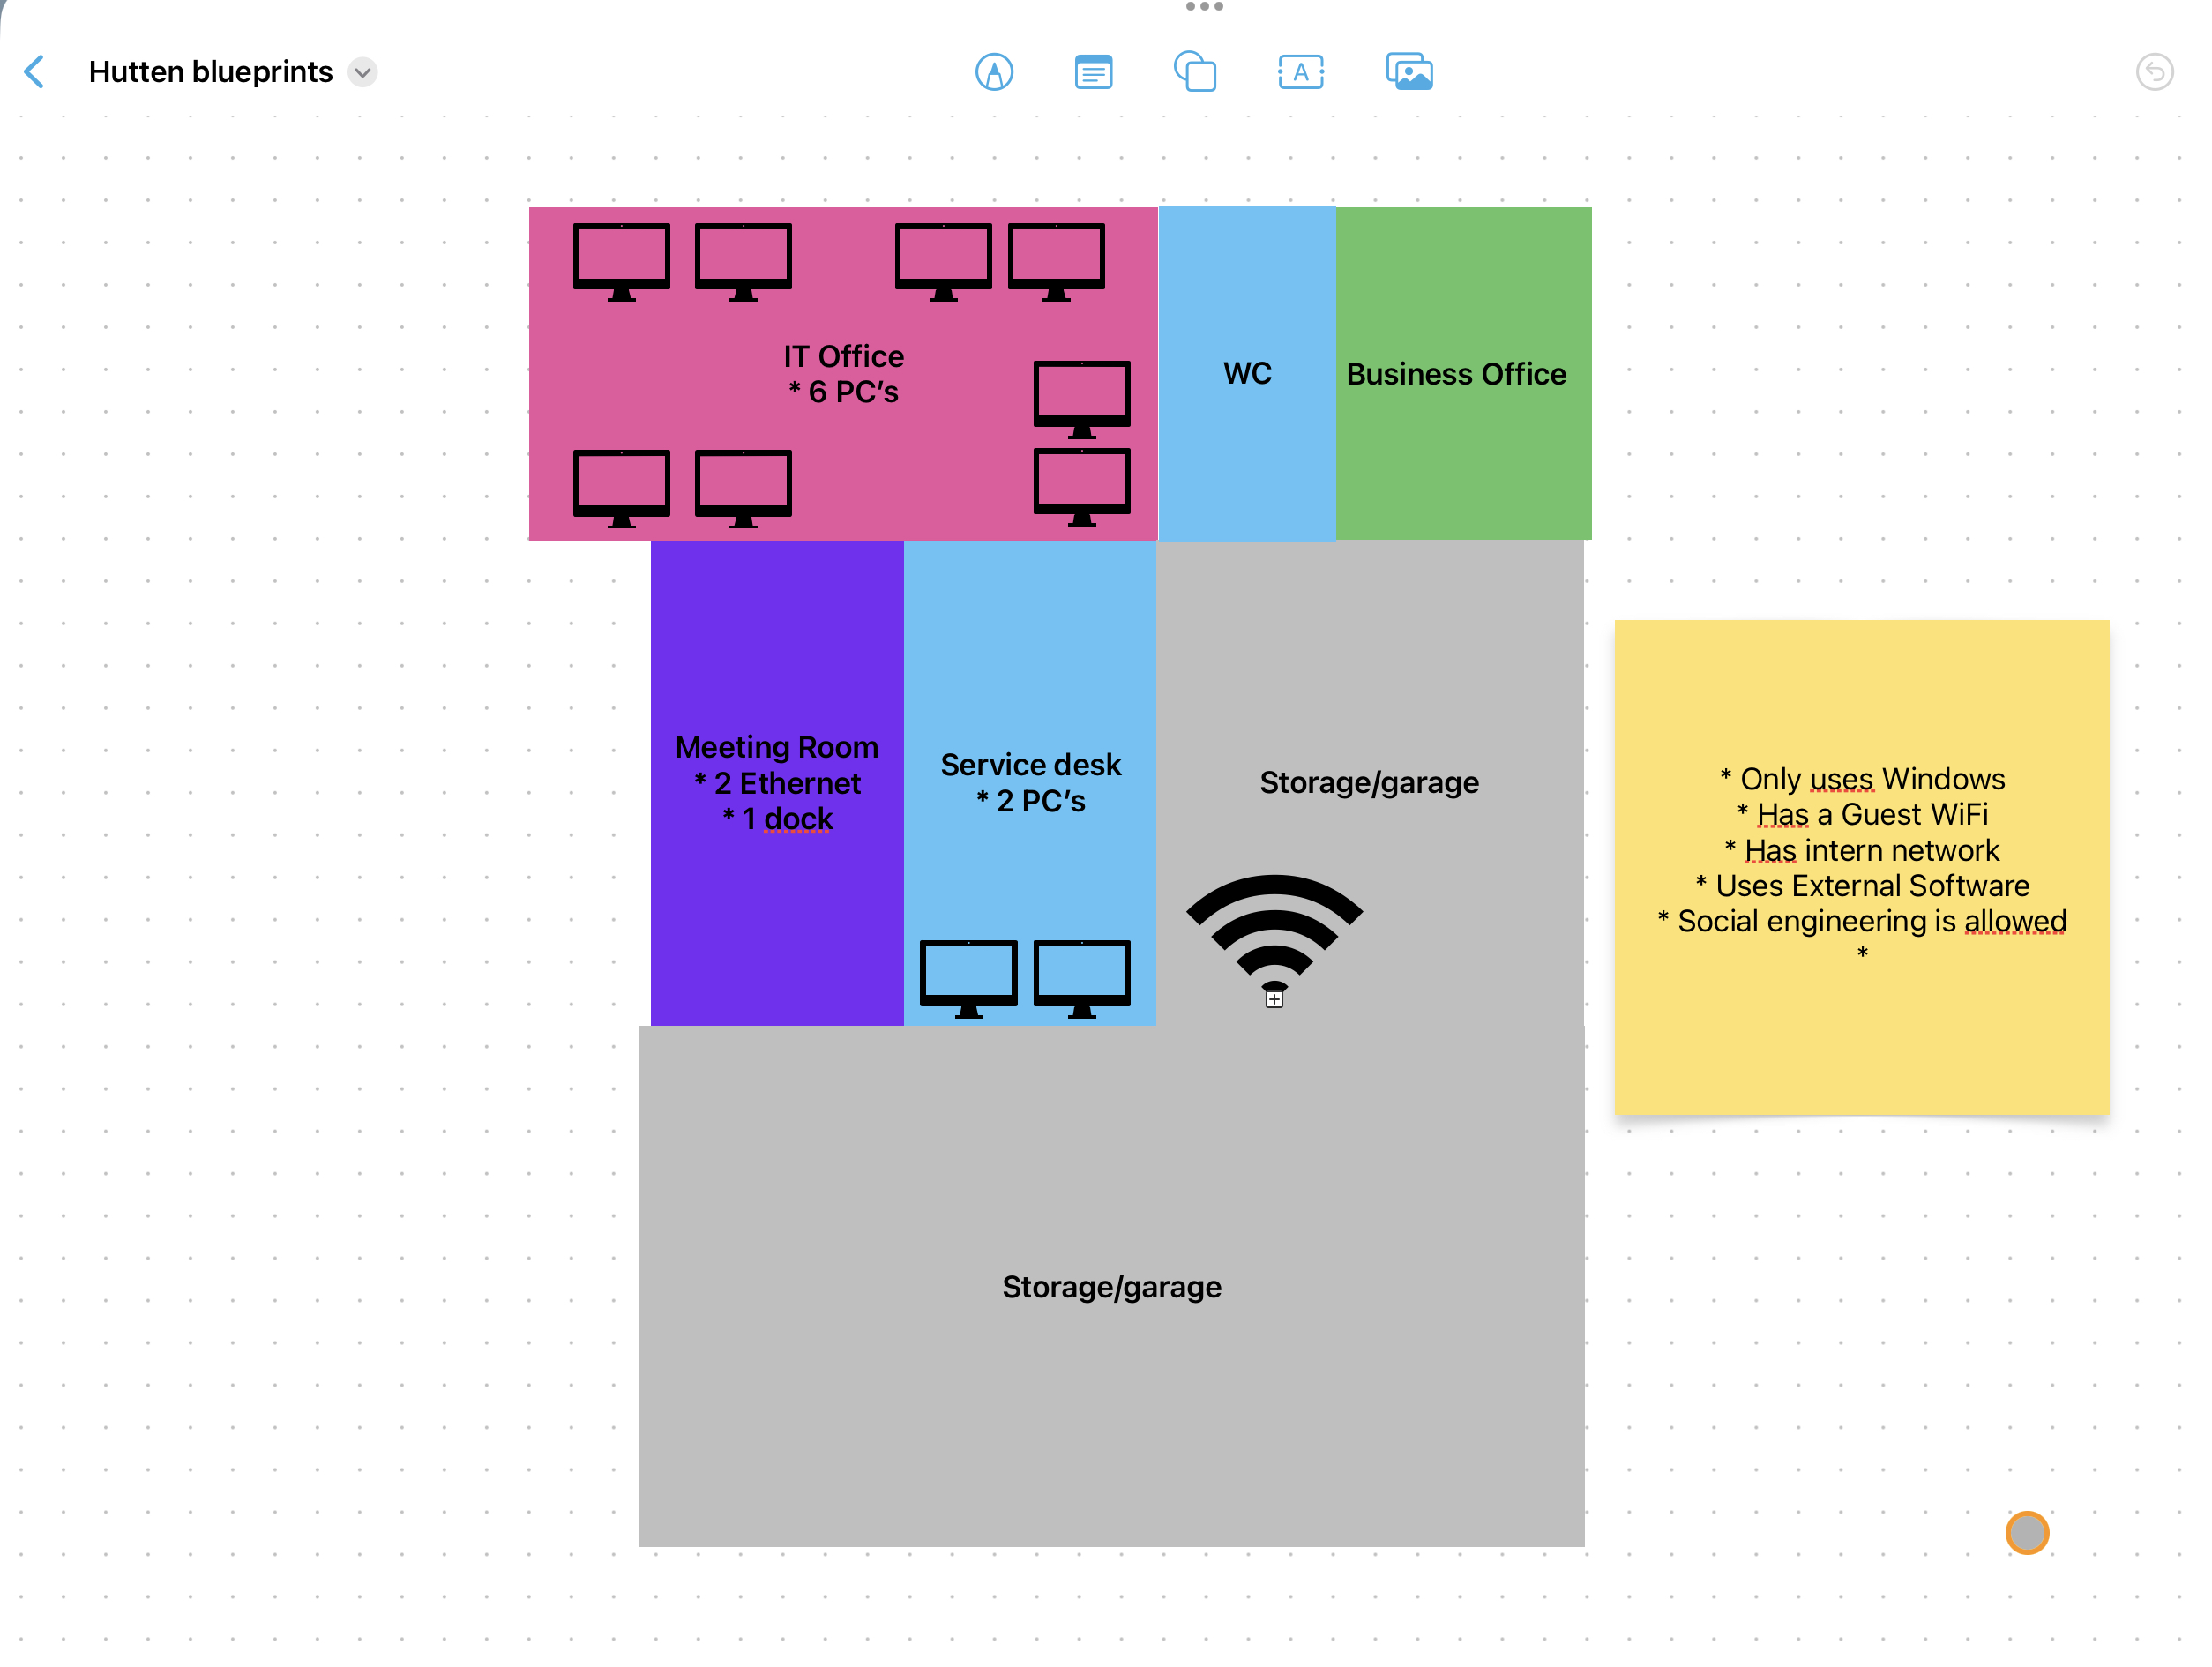
\includegraphics[width=0.8\textwidth]{fotos/Portfolio/Huttenblueprint.jpeg}
\hfill\break
\textbf{LO2 Risk Consultant}
\hfill\break
With our client, we've discussed the possible outcomes and the risk that comes with it like finding a password which means that they need to change their password and we may find some personal information from their former colleagues. But this will be handled professionally.
\hfill\break
\textbf{LO3 Security Engineer}
\hfill\break
I, Dean and Konstantin have compiled a Group and Penttesting agreement/contract and we keep our promises at least I do and I enforce others to do the same since I have their signatures in Teams doc.
\hfill\break
\textbf{LO4 Security Analyst}
\hfill\break
We caref-ully discussed our options within the group and tried to make leas as possible noise into our network.
\hfill\break
\textbf{LO5 Security Professional}
\hfill\break
I stood ready to communicate between our client and the group not only that I was most of the time at our pen-testing and was there till the end.
\item \textbf{What are you proud of?}
\hfill\break
That I went full Footprinting mode into our first meeting. I've mapped their whole IT with all possible ports, laptops, Computers, and operating systems just by looking around and talking/ asking sneaky questions to them. Even the teachers were impressed with how much info I got and noted into my notes and drew a small map into my iPad Pro.
\item \textbf{Which aspects do you want to develop further?}
\hfill\break
\hfill\break
I think I've mastered the Social engineering part so I want to actually focus more on the exploit part where we trick the employees with our fake mail and create an API to mimic webmail so we can fish him. That would be cool and I made a mailing system + API in golang so I can continue developing that.
\item \textbf{What will you do differently next time?}
\hfill\break
\hfill\break
To be more prepared with the group or at least to do proper preparation. Ask about their main software so that we could search for CVEs before our first day.
\item \textbf{What grade would you give yourself on the corresponding Learning Outcome?}
\hfill\break
Even though I did a lot of social engineering and helped Dean with our fishing mail I have a feeling I didn't do a lot so I would pick a solid proficient.
\end{itemize}

\newpage
\subsection{Security Engineer and Security Analyst (Blue/Defending)}
\begin{itemize}
\item \textbf{What did you do in this project?}
\hfill\break
Did planning, and was in charge of documenting the whole document plus adding pictures and adding text while my classmates were busy, Creating 2 DC and a backup DC, and helped guide with AD RBAC, guided the group when the team leader was struggling.
\item \textbf{How did you apply your skills in the project?}
\begin{itemize}
    \item Threat + Risk Analysis pt1 CIA
    \item Identity Management, Authentication and Access Control
    \item Network Separation and Segmentation
    
\end{itemize}
\item \textbf{What have you learned considering this Learning Outcome?}
\break
\textbf{LO2 Risk Consultant}

\textbf{LO3 Security Engineer}
\hfill\break
Creating a backup strategy and discussing it with our group.
\hfill\break
\textbf{LO4 Security Analyst}

\textbf{LO5 Security Professional}
\hfill\break
Holding a Scrum and planning and dividing the tasks.
\hfill\break
\item \textbf{What are you proud of?}
\hfill\break
Not much here since here I'm not a project leader anymore. So I sat and listened to our project leader. My role was more of an fall back leader so I if something wasn't done or finished I step in and guide our group until we were stable.
\hfill\break
\item \textbf{Which aspects do you want to develop further?}
\hfill\break
To be more flexible in the group like a Scrum master or note taker. Okay scrum master maybe not be the best example since I did that but we didn't use Trello or any other boards. We kept it in Discord or Teams and every planning was just inside my head or in my calendar. I know that my teammates did not care for planning since we already knew what we had to do and what our deadlines were.
\hfill\break
\item \textbf{What will you do differently next time?}
Maybe step in sooner since our current project leader is an introvert(which isn't bad) but he was nervous and was afraid to do stand-ups now we are in a Mexican stand-off over who to blame and our project went bad. To be honest it was my fault to step down as a leader now that everyone got used to my method of working.
\item \textbf{What grade would you give yourself on the corresponding Learning Outcome?}
\hfill\break
Proficient since my input wasn't big compared to pen testing.
\end{itemize}

\newpage
\subsection{Security Professional}
\begin{itemize}
\item \textbf{How did you obtain Body of Knowledge* about the involved subjects? (note: just a summary needed here; what were your favorite subjects, overall impression? You can refer to the BoK-document section)}
\begin{itemize}
    \item Footprinting, Reconnaissance and Social Engineering
    \item Law \& Ethics and Responsible Disclosure + GDPR
\end{itemize}
In the beginning, we had to command inject the code in a week (titel van command injection). (insert opdracht met Philips footprinting), 
\item \textbf{How did you apply your skills in the project?}
\hfill\break
\hfill\break
Just to be on time for school and be present every school day. And submit your documents on Tuesday every time so that my teachers can give feedback in the morning.
\item \textbf{What have you learned considering this Learning Outcome?}
\break
\textbf{LO3 Security Engineer}
\hfill\break
Creating a secure solution where I created a Disaster Plan.
\hfill\break
\textbf{LO4 Security Analyst}
\hfill\break
Creating analysis for backup strategy and still researching alongside Dean(Open Sense) and Konstantin (RBAC)
\hfill\break
\textbf{LO5 Security Professional}
\hfill\break
I've been always focused to be on time and always communicating with everyone and every platform(Teams and Discord) the proof is on Teams and other teachers can view our group-h chat.
\item \textbf{What are you proud of?}
\hfill\break
\hfill\break
The thing that I was proud of is that I did not lazy with my homework and submitted it on regular bases. Because I had issues in the previous semesters I had a good start at the beginning of the semester then I fell between satisfactory and unsatisfactory.

In short, I'm more accustomed to Fontys rhythm which means I can be more consistent with my work which I'm most proud of.
\hfill\break
\hfill\break
Plus I got friendly feedback to be a great leader and a team player.
\hfill\break
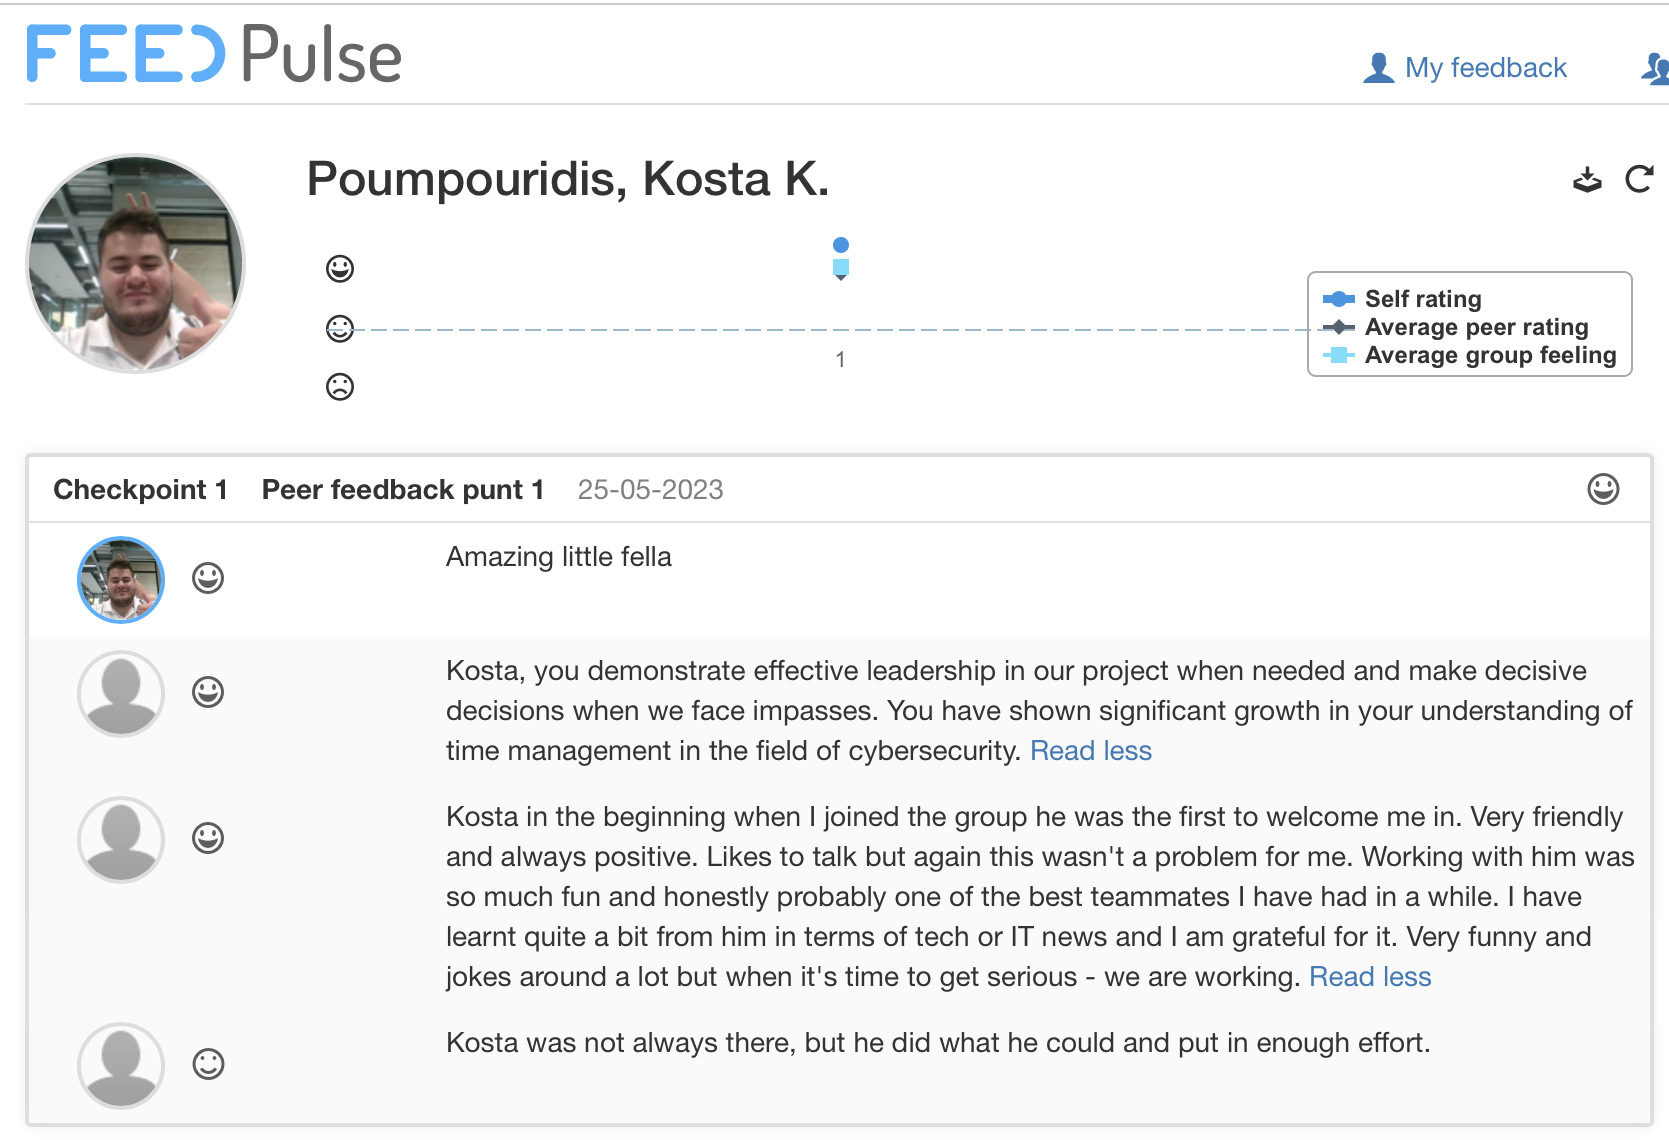
\includegraphics[width=0.8\textwidth]{fotos/Portfolio/Feedpulse.jpeg}
\break
\emph{Feedback from my group H}
\item \textbf{Which aspects do you want to develop further?}
To be more time efficient because now almost the end of the semester I have been slacking off a bit because I'm not the leader anymore which means I'm taking no responsibilities and that made me mellow. I need to be efficient even at the end of the semester.
\item \textbf{What will you do differently next time?}
\hfill\break
\hfill\break
Not much really. I'm studying since MBO 2 and went to 3, 4 and now in HBO. I've had enough time to reflect upon my discipline.
\item \textbf{What grade would you give yourself on the corresponding Learning Outcome?}
\hfill\break
\hfill\break
What kind of question is that? Of course an outstanding! But all jokes aside I think a satisfactory or an advance since I've been very active this semester and did some advanced challenges at the beginning of the semester. Maybe in between?
\end{itemize}

\newpage
\section{Personal Projects}
\begin{itemize}
\item How did you spend your hours for:
\begin{itemize}
\item \textbf{Personal Vulnerability Investigation (expected about 5x4h = 20 hours)}
\hfill\break
\hfill\break
First I needed to propose the subject. Hacking SMBv1 with Fritzbox and made a small proposal before starting to take materials from home and starting the research.
\item \textbf{Internship Preparation (expected about 10 hours)}
\hfill\break
\hfill\break
Apparently, I skipped this by accident because they sent a mail like etiquette and I thought it was spam so I ignored it. But I'm happy to announce that:
\begin{enumerate}
    \item Updated my \textbf{\href{https://www.linkedin.com/in/kostapoum/}{LinkedIn (link)}}
    \item Have an \textbf{\href{https://poumpouridis.carrd.co}{ e-business card (link)}}
    \item Went to carrier day in Fontys Strijp S
\end{enumerate}
\item Personal Specialisation Project (expected about 10x4h = 40 hours)
\hfill\break
\hfill\break
Oof. I don't remember anymore because I started somewhere in February and made a proof of concept somewhere in May. I have proven in some forums that I had a working config for my PSP but I think I've put more than 40 hours on research alone. and building a working config took me 2 weeks to make it work.
\hfill\break
\hfill\break
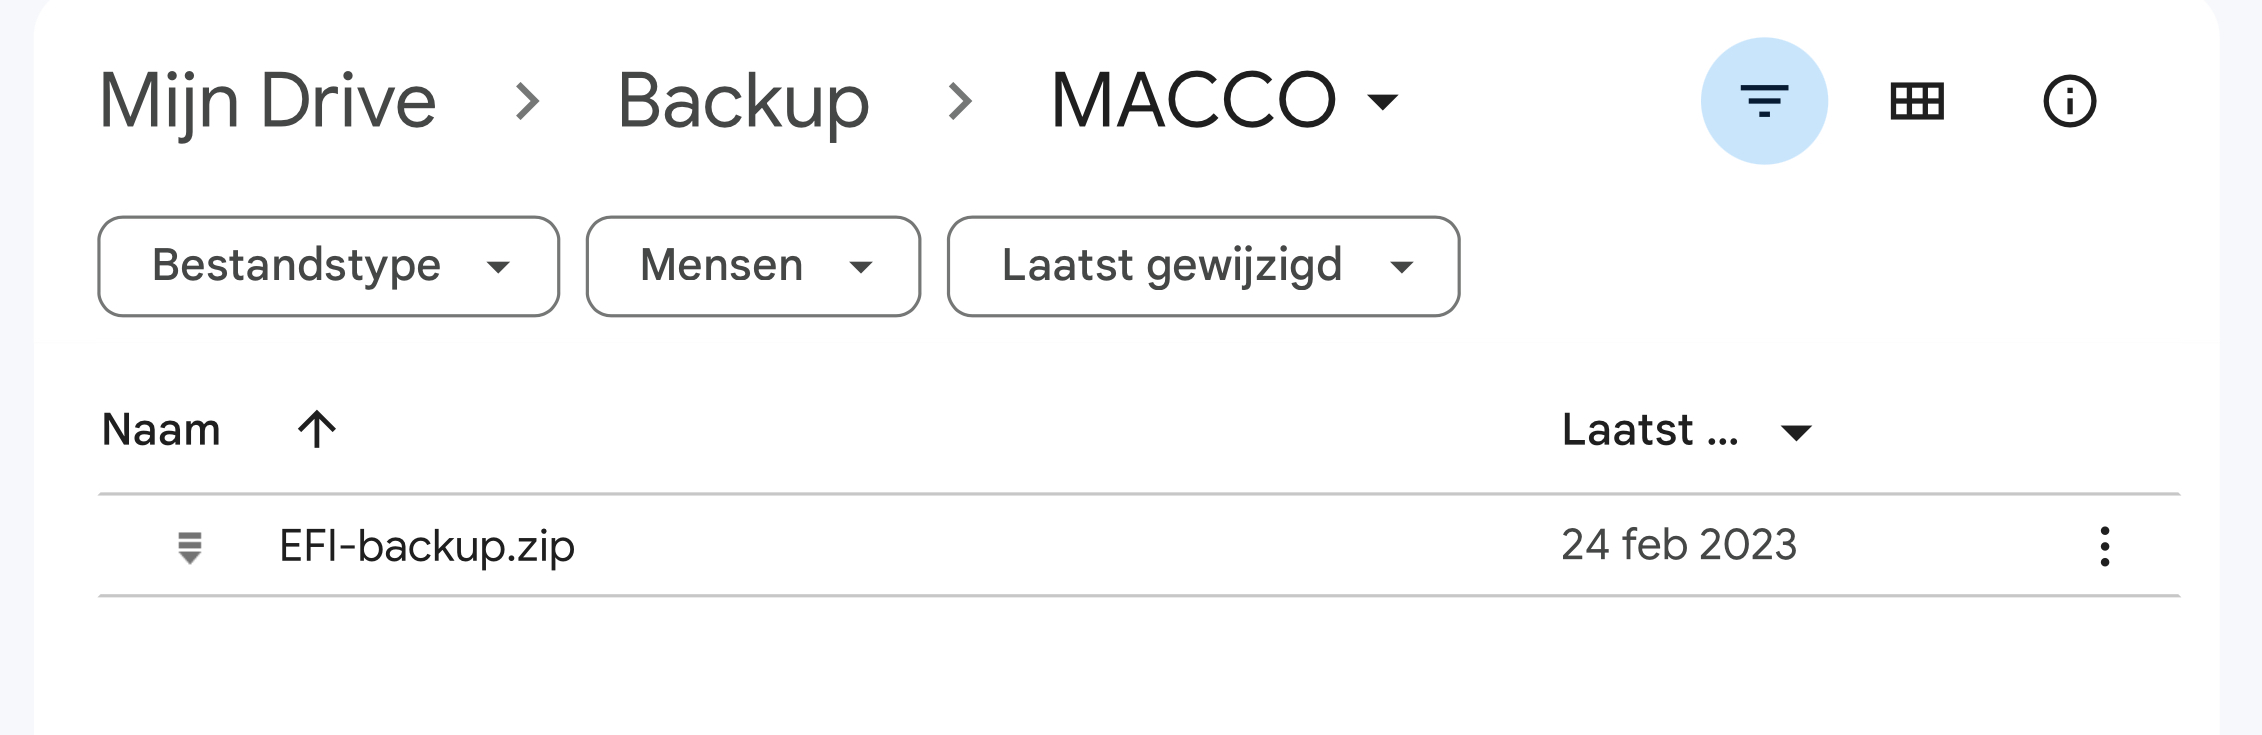
\includegraphics[width=0.8\textwidth]{fotos/Portfolio/Gdrive Marco backup.jpeg}
\end{itemize}
\end{itemize}

\newpage
\section{Overall Conclusion and Reflection}
To be honest I felt that I've grown a lot with my work and pace. Maybe because back then I had more free time for school or had amazing classmates to push through homework. 
\hfill\break
\hfill\break
I did not grow as much as my group but I was steadily growing. Of course, I wasn't perfect because even though my PVI and PSP went well I struggled a lot and did not document all of it so I can improve that. 
\hfill\break
\hfill\break
If I have to compare myself from week 1 to the end of the semester. To be honest, what can I say? I was a driving force like Dean. We both did some advanced challenges (He did more I guess). Maybe I was less annoying to the teacher since later in the semester I read the canvas instead of asking a question every minute. But in all seriousness I went from Leading the group to teaching someone to lead a group I guess my inner teaching comes alive hahaha.


\end{document}